\chapter{Quantum Computing Overview }
\graphicspath{ {./images/} }

\[ \boxed {\mbox{i\textbf{h}}\dfrac{\partial}{\partial t}|\psi(t)\rangle = \bm{\hat{\textnormal{\bfseries H}}} |\psi(t)\rangle }
\]

Quantum Computing \cite{QCQI} is doing computation using quantum-mechanical phenomena like superposition and entanglement. A Quantum computer performs such computing and is very different from a classical computer that depends on digital logics and transistors. Quantum computation uses Quantum bits also called \textit{Qubits} which align in different ways to produce variations of not just 1 or 0 (as in classical computing) but many others. An approximation based on probability of outcome which depends on solving governing physics equations, theoretically allows us to construct subsequent logic of state or data changes.\\

A Quantum Turing Machine is theoretical accepted model of quantum computer which has been made possible by the initial works of \textbf{Richard Feynman}, \textbf{David Deutsch}  and \textbf{Yuri Manin}. The actual implemtation model of the quantum computer however is still in a very basic phase because of very absurd Temperature-Pressure conditions required to maintain a very less stable qubit state. The current research in quantum computing hardware focuses on precisely maintaining qubit's state and reducing data loss during state transition. The implementational software aspect of quantum computer is explored even smaller much because of less compatible quantum hardware and the inability of classical computers to simulate large qubit quantum computer.\\

\section{Qubits}
Quantum bits or Qubits are quantum version of classical binary bit. It is the basic unit of quantum information. Unlike the classical bits the Qubit can maintain information in unique states or in a superposition of states or may be  entangled states. The possiblity of having so many states improves the parallelism of data computaion and hence speed. A very good example is often potrayed by finding the card in which given 4 cards with one card different, we need to find the odd one out. The classical computer takes a maximum of 4 steps but a quantum computer will take always only 1 step to figure it out. 

\subsection{Representation}
Quantum State refers to the state of isolated quantum system. It gives a basic idea of possibility of different observable outcomes. A Qubit state can be represented by conventional "Dirac" or "bra-ket" notation, written as $|0\rangle$ or $|0\rangle$ and read as "ket-0" or "ket-1". two orthonormal \textit{Basis States} \{ $|0\rangle$ , $|1\rangle$ \} form 2-D linear vector space of qubit. Qubit basis states combine together to form \textit{Product Basis Space} like,

\[ |00\rangle = \begin{bmatrix} 1 \\ 0 \\ 0 \\ 0 \end{bmatrix} \quad \\
   |01\rangle = \begin{bmatrix} 0 \\ 1 \\ 0 \\ 0 \end{bmatrix} \quad \\
   |10\rangle = \begin{bmatrix} 0 \\ 0 \\ 1 \\ 0 \end{bmatrix} \quad \\
   |11\rangle = \begin{bmatrix} 0 \\ 0 \\ 0 \\ 1 \end{bmatrix} \quad \\
\]

A pure qubit state is a coherent superposition of the basis states. This means that a single qubit can be described by a linear combination of $|0\rangle$ \& $|1\rangle$.

\[|\psi\rangle = \alpha|0\rangle \quad +\quad \beta|1\rangle\]

with condition that 

\[\alpha^2 + \beta^2 = 1\ \cdots (i) \].

The probabilities of finding states of values $|0\rangle$ \& $|1\rangle$ is proportional to $|\alpha|^2$ and $|\beta|^2$ respectively.\\

The other type of representation is called \textbf{Bloch Sphere Representation} in which $\alpha$ and $\beta$ are considered as complex numbers with two degrees of freedom and a normalization constraint of equation (i). 

\begin{figure}[!htb]
\centering
  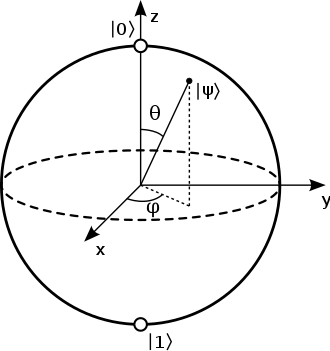
\includegraphics[scale=0.5]{bloch}
  \caption{Bloch Sphere Representation of a Qubit (source : The Quantum Computing \& Quantum Information book)}
\end{figure}

\[\alpha =  e^{i\psi}cos\dfrac{\theta}{2} \quad \& \quad \beta = e^{i(\psi + \phi)}sin\dfrac{\theta}{2} \].

\subsection{Quantum Superposition}
Superposition is essentially the ability of a quantum system to be in multiple states at the same time — that is, something can be “here” and “there,” or “up” and “down” at the same time.

\subsection{Quantum Entanglement}
It is a physical phenomena which that is said to occur when pairs or groups of particles are generated or they interact or share same spatial proximity such that behaviour of any one of the particles can not be defined independently of the state of others. Entanglement is an extremely strong correlation that exists between quantum particles — so strong, in fact, that two or more quantum particles can be inextricably linked in perfect unison, even if separated by great distances. The particles remain perfectly correlated even if separated by great distances. The particles are so intrinsically connected, they can be said to “dance” in instantaneous, perfect unison, even when placed at opposite ends of the universe. This seemingly impossible connection inspired Einstein to describe entanglement as "\underline{spooky action at a distance}".

\section{Quantum Gates \& Circuits}
A quantum gate or quantum logic gate is a rudimentary quantum circuit operating on a small number of qubits. They are the analogues for quantum computers to classical logic gates for conventional digital computers. \underline{Quantum logic gates are reversible}, unlike many classical logic gates. Some universal classical logic gates, such as the Toffoli gate, provide reversibility and can be directly mapped onto quantum logic gates. Quantum logic gates are represented by unitary matrices. The action of the gate on a specific quantum state is found by multiplying the vector which represents the state by the matrix representing the gate.\\


\begin{figure}[!htb]
\centering
  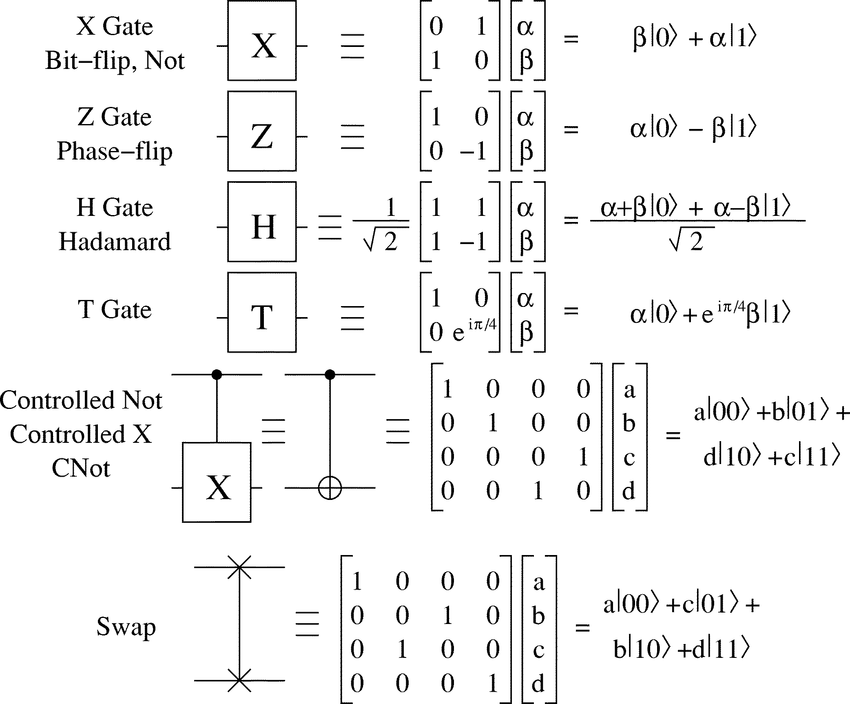
\includegraphics[scale=0.4]{qgates}
  \caption{Some common Quantum Logic gates (source: wikipedia)}
\end{figure}

A \textbf{Quantum Circuit} is an ordered logical combination of quantum gates and some initial Qubits. The quantum circuits are reversible transformations on a quantum mechanical analog of an n-bit register. It is very important for any logic circuit to be reversible to return n bit data output for a n bit data input. In other words the reversible logic gates are bijective mappings from a n bit data set to itself. \textbf{Kitaev} mentioned that irreversible circuits increase the physical entropy of the system. Theoretical advancements showed that \textbf{Toffoli Gate} is a Universal reversible Gate. this basically mean that we can easily consruct a large sizes circuit by simply adding more gates (Toffoli gates as example here) to it.

\begin{figure}[!htb]
\centering
  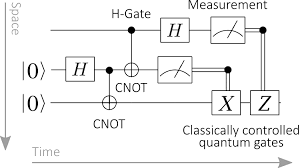
\includegraphics{qcircuit}
  \caption{An example of a quantum circuit (source : The Quantum Computing \& Quantum Information book) }
\end{figure}

\subsection{Error Correction}
Error Corection is very important for scalibility of a quantum computer. An error correction of $10^{-2}$ means we can add atmost 100 logic gates before running into complete mess and even destroying the qubit chip. Research going on is trying to reduce this error correction to as low as possible.




